\chapter{Kvalitetssikring}\label{ch:Kvalitetssikring}

I dette afsnit er det set på, hvordan gruppen har kvalitetssikret projektet ud fra brug af XP og FURPS+. 




\section{FURPS+ Og XP}


Som nævnt tidligere fokuserer agile udviklingsmetoder knap så meget på dokumentation, men mere på selve udviklingen af softwaren. Alt dokumentation, som ikke har en direkte indflydelse på softwaren, bliver nedprioriteret. Kvalitet i softwareudvikling omhandler koden mere end det gør andet. Kvalitetssikring kan beskrives ud fra FURPS+\cite{furps}. FURPS er Functionality, Usability, Reliability, Performance og Supportability. I dette projekt er der lavet refactoring, som er omskrivning af kode, så det bliver nærmere at læse, og Test Driven Development har været en central del af projektet. Gruppen har tidligere besluttet at benytte procedurer fra XP til udviklingen af dette projekt, så procedurer som Pair Programming, Simple Design, Refactoring og Planning Game har gruppen sørget for at kvalitetssikre produktet. Til dette har Pair Programming haft en stor indflydelse på kvaliteten af produktet, da det leder til en dybere forståelse af et produkt. \cite{Sommerville}


\begin{figure}
    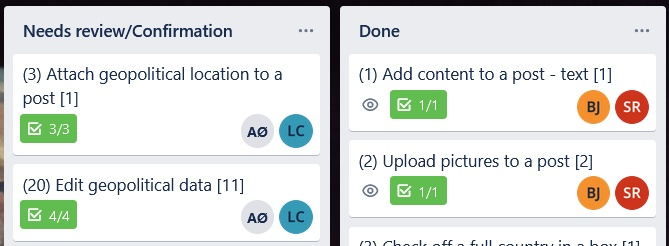
\includegraphics[width=\linewidth]{figures/pairprogramming.jpg}
    \caption{Ekempel af hvordan gruppen har benyttet Pair Programming fra XP.}
    \label{fig:Pair}
\end{figure}



\begin{figure}
    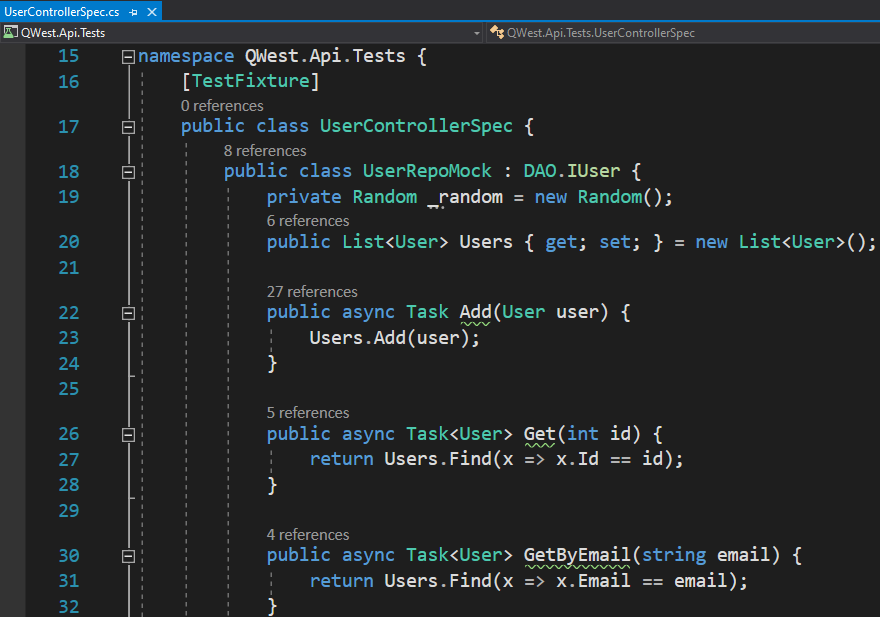
\includegraphics[width=\linewidth]{figures/tests.png}
    \caption{Eksempel på test.}
    \label{fig:Test}
\end{figure}


\begin{figure}
    
\includegraphics[width=\linewidth]{figures/planningpoker.jpg}
    \caption{Ekempel på hvordan Planning Poker er benyttet gennem hele projektet.}
    \label{fig:Poker}
\end{figure}